\documentclass[11pt,a4paper]{article}
\usepackage[T1]{fontenc}
\usepackage{lmodern}
\usepackage[margin=2.2cm]{geometry}
\usepackage{microtype}
\usepackage{booktabs}
\usepackage{graphicx}
\usepackage[font=small,labelfont=bf,skip=4pt]{caption}
\usepackage{subcaption}
\usepackage{xcolor}
\usepackage{float}
\usepackage{enumitem}
\usepackage[colorlinks=true,linkcolor=blue!50!black,urlcolor=blue!50!black]{hyperref}
\setlength{\parskip}{0.45em}
\setlength{\parindent}{0pt}
\renewcommand{\arraystretch}{1.12}
\newcommand{\note}[1]{\textcolor{black!60}{\small #1}}

\title{Mining GitHub for Metamorphic Testing:\\ Shared Data for the Final Report}
\date{16 October 2026}
\author{}
\begin{document}
\maketitle
\vspace{-2em}

\section*{About the data}
\begin{itemize}[leftmargin=1.2em,itemsep=1pt]
\item \textbf{Search.} GitHub search on six surfaces (code, repositories, commits, pull requests, issues, discussions), 2010-01-01 to 2026-09-01. Only explicit technique phrases count; for MT the keyword \texttt{"@metamorphic"} is excluded (GitHub ignores the \texttt{@} and searches the bare word).
\item \textbf{Verified results only.} A non-code result counts only if its title or body contains a technique phrase; a code-surface repository counts only if its current snapshot contains one. Everything else is treated as not found.
\item \textbf{Current state.} Repositories were re-scanned on their current default-branch snapshot (October 2026); repositories deleted or made private since the search are excluded.
\item \textbf{PBT and fuzz} have 76,846 and 255,740 code-surface repositories, so their cloning-based figures use seeded random samples sized for $\pm$3\% at 95\% confidence (PBT: 1,112 analysed; fuzz: 1,140 analysed). Their commit searches hit GitHub's 1{,}000-results-per-query cap; the timeline figures use the corrected counts (exact for PBT, estimated with 95\% confidence intervals for fuzz).
\item \textbf{2026} covers January--August only (search ended 2026-09-01), marked with * in the figures.
\end{itemize}

\section{RQ1 -- Adoption: how much is metamorphic testing used?}

\begin{table}[htbp]
\centering
\small
\caption{Metamorphic testing on GitHub: search hits and distinct repositories per search surface (S1, S2).}
\label{tab:mt-search}
\begin{tabular}{@{}lrrr@{}}
\toprule
Surface & Search hits & Verified results & Distinct repositories \\
\midrule
Code & 49,948 & 28,268 & 5,879 \\
Repositories & 848 & 230 & 230 \\
Commits & 24,754 & 4,160 & 1,156 \\
Pull requests & 8,442 & 1,169 & 507 \\
Issues & 5,213 & 1,175 & 453 \\
Discussions & 78 & 16 & 8 \\
\midrule
\textbf{All surfaces} &  &  & \textbf{7,060} \\
\bottomrule
\end{tabular}
\par\smallskip\parbox{0.94\linewidth}{\footnotesize Search hits: GitHub's reported \texttt{total\_count} summed over the search keywords (before de-duplication). Verified results: distinct items whose text (non-code) or repository snapshot (code) contains an MT phrase. A repository found on several surfaces is counted once in the total.}
\end{table}

\paragraph{Size of the code-surface repositories (S3).} The 5,879 verified code-surface repositories contain 28,801,574 files in total, of which 5,330,852 are code files with 1,710~million lines of code (median per repository: 79 code files, 17,964 lines of code).

\paragraph{Keywords without results (S4).} All 18 search keywords returned results on the code and commits surfaces. Interestingly, some keyword forms are never seen elsewhere: on the repositories surface \texttt{metamorphic groups}, \texttt{metamorphic oracle}; on the pull requests surface \texttt{metamorphic\_relation}, \texttt{metamorphic\_tests}; on the issues surface \texttt{metamorphic\_relation}, \texttt{metamorphic\_relations}; on the discussions surface \texttt{metamorphic relation}, \texttt{metamorphic relationship}, \texttt{metamorphic relationships}, \texttt{metamorphic group}, \texttt{metamorphic groups}, \texttt{MetamorphicTest}, \texttt{MetamorphicRelation}, \texttt{metamorphic\_relation}, \texttt{metamorphic\_relations}, \texttt{metamorphic\_test}, \texttt{metamorphic\_tests}. The identifier forms (e.g.\ \texttt{metamorphic\_relation}) are essentially code-only.

\paragraph{Technique keywords (A1).} In the code of the 5,879 repositories, the most frequent forms are \emph{metamorphic test(ing)} (46,334 lines in 4,370 repositories), \emph{metamorphic relation} (28,358 lines in 2,346 repositories), \emph{metamorphic\_test* (snake\_case)} (17,599 lines in 372 repositories). In the 6,750 verified issues, pull requests, commits, discussions and repository descriptions, the leading forms are \emph{metamorphic test(ing)} (4,397 items), \emph{metamorphic relation} (1,679 items), \emph{metamorphic property} (650 items).

\section{RQ2 -- Usage and classification}

\paragraph{Usage vs.\ non-usage (A2).} Of the 6,117 code-surface repositories found by the search, 5,879 still contain an MT phrase today (excluded: 146 deleted or private, 90 no longer containing a phrase, 2 could not be scanned). \textbf{1,677 (28.5\%) are \emph{usage} repositories}, with a technique phrase in at least one code file; 4,202 (71.5\%) mention MT only outside code (documentation, configuration, data).

\begin{table}[htbp]
\centering
\small
\caption{Code files of the 1,677 MT usage repositories (A3).}
\label{tab:mt-a3}
\begin{tabular}{@{}lrrrr@{}}
\toprule
Code-file category & Mean \% per repo & Median \% & Files & \% of all files \\
\midrule
Technique test files & 1.3\% & 0.1\% & 3,702 & 0.2\% \\
Other test files & 26.3\% & 25.0\% & 568,103 & 25.3\% \\
Technique non-test code files & 4.1\% & 0.1\% & 3,333 & 0.1\% \\
Other non-test code files & 68.3\% & 69.9\% & 1,671,337 & 74.4\% \\
\bottomrule
\end{tabular}
\par\smallskip\parbox{0.94\linewidth}{\footnotesize \emph{Technique} = the file contains an MT phrase or identifier. Test files: test-file naming conventions (e.g.\ \texttt{test\_*.py}, \texttt{*Test.java}, \texttt{*.spec.ts}), pytest/JUnit imports or \texttt{@Test}, or a test/spec directory. Mean and median are taken over repositories.}
\end{table}

\paragraph{Non-usage repositories (A4).} In the 4,202 non-usage repositories, MT appears in 2.9\% of documentation files and 1.0\% of other non-code files on average, i.e.\ typically in a handful of README, notes or data files.

\begin{table}[htbp]
\centering
\small
\caption{Primary language of the MT code-surface repositories, normalised by GitHub-wide popularity (A5).}
\label{tab:mt-a5}
\begin{tabular}{@{}lrrrr@{}}
\toprule
Language & Repositories & MT share & GitHub share & Lift \\
\midrule
Python & 2,061 & 38.3\% & 18.89\% & \textbf{2.03} \\
TypeScript & 585 & 10.9\% & 13.61\% & 0.80 \\
HTML & 525 & 9.7\% & 24.52\% & 0.40 \\
Rust & 426 & 7.9\% & 0.82\% & \textbf{9.61} \\
JavaScript & 394 & 7.3\% & 16.29\% & 0.45 \\
Jupyter Notebook & 233 & 4.3\% & 4.27\% & 1.01 \\
TeX & 209 & 3.9\% & 0.17\% & \textbf{23.11} \\
C++ & 165 & 3.1\% & 2.30\% & 1.33 \\
Go & 150 & 2.8\% & 1.07\% & \textbf{2.61} \\
Java & 127 & 2.4\% & 5.03\% & 0.47 \\
Shell & 100 & 1.9\% & 1.35\% & 1.38 \\
C & 57 & 1.1\% & 1.33\% & 0.80 \\
C\# & 57 & 1.1\% & 2.16\% & 0.49 \\
CSS & 52 & 1.0\% & 3.66\% & 0.26 \\
R & 29 & 0.5\% & 0.31\% & 1.75 \\
\bottomrule
\end{tabular}
\par\smallskip\parbox{0.94\linewidth}{\footnotesize Both shares are taken over the 30 languages with a GitHub-wide count: MT share = of the 5,386 MT repositories in those languages; GitHub share = of the 73,255,947 public repositories in those languages pushed since 2025-09-01 (GitHub repository search). Lift = MT share $\div$ GitHub share; values above 1 mean the language is over-represented among MT repositories (bold: $\geq 2$).}
\end{table}

\begin{table}[htbp]
\centering
\small
\caption{Application domain of the 1,948 repositories with a verified non-code MT result (A6).}
\label{tab:mt-a6}
\begin{tabular}{@{}lrrrr@{}}
\toprule
Domain & \shortstack{Description\\+ topics} & \% & \shortstack{+ README} & \% \\
\midrule
Web / APIs & 83 & 4.3\% & 357 & 18.3\% \\
Machine learning & 227 & 11.7\% & 349 & 17.9\% \\
Databases & 92 & 4.7\% & 331 & 17.0\% \\
Compilers / programming languages & 100 & 5.1\% & 178 & 9.1\% \\
Security / cryptography & 69 & 3.5\% & 170 & 8.7\% \\
Scientific computing & 84 & 4.3\% & 131 & 6.7\% \\
Operating systems & 38 & 2.0\% & 131 & 6.7\% \\
Finance & 65 & 3.3\% & 108 & 5.5\% \\
Autonomous systems / robotics & 46 & 2.4\% & 61 & 3.1\% \\
Distributed systems & 36 & 1.8\% & 56 & 2.9\% \\
Embedded / IoT & 24 & 1.2\% & 32 & 1.6\% \\
Bioinformatics & 13 & 0.7\% & 16 & 0.8\% \\
\midrule
\emph{No domain matched} & 1,317 & 67.6\% & 869 & 44.6\% \\
\bottomrule
\end{tabular}
\par\smallskip\parbox{0.94\linewidth}{\footnotesize Keyword matching against an ACM CCS-based domain vocabulary (whole words). Description + topics: any domain keyword; + README: the README adds a domain only if it contains at least three different keywords of that domain. A repository can have several domains. Heuristic; ten random repositories per domain are listed for manual checking.}
\end{table}

\begin{figure}[htbp]
\centering
\begin{subfigure}{\linewidth}\centering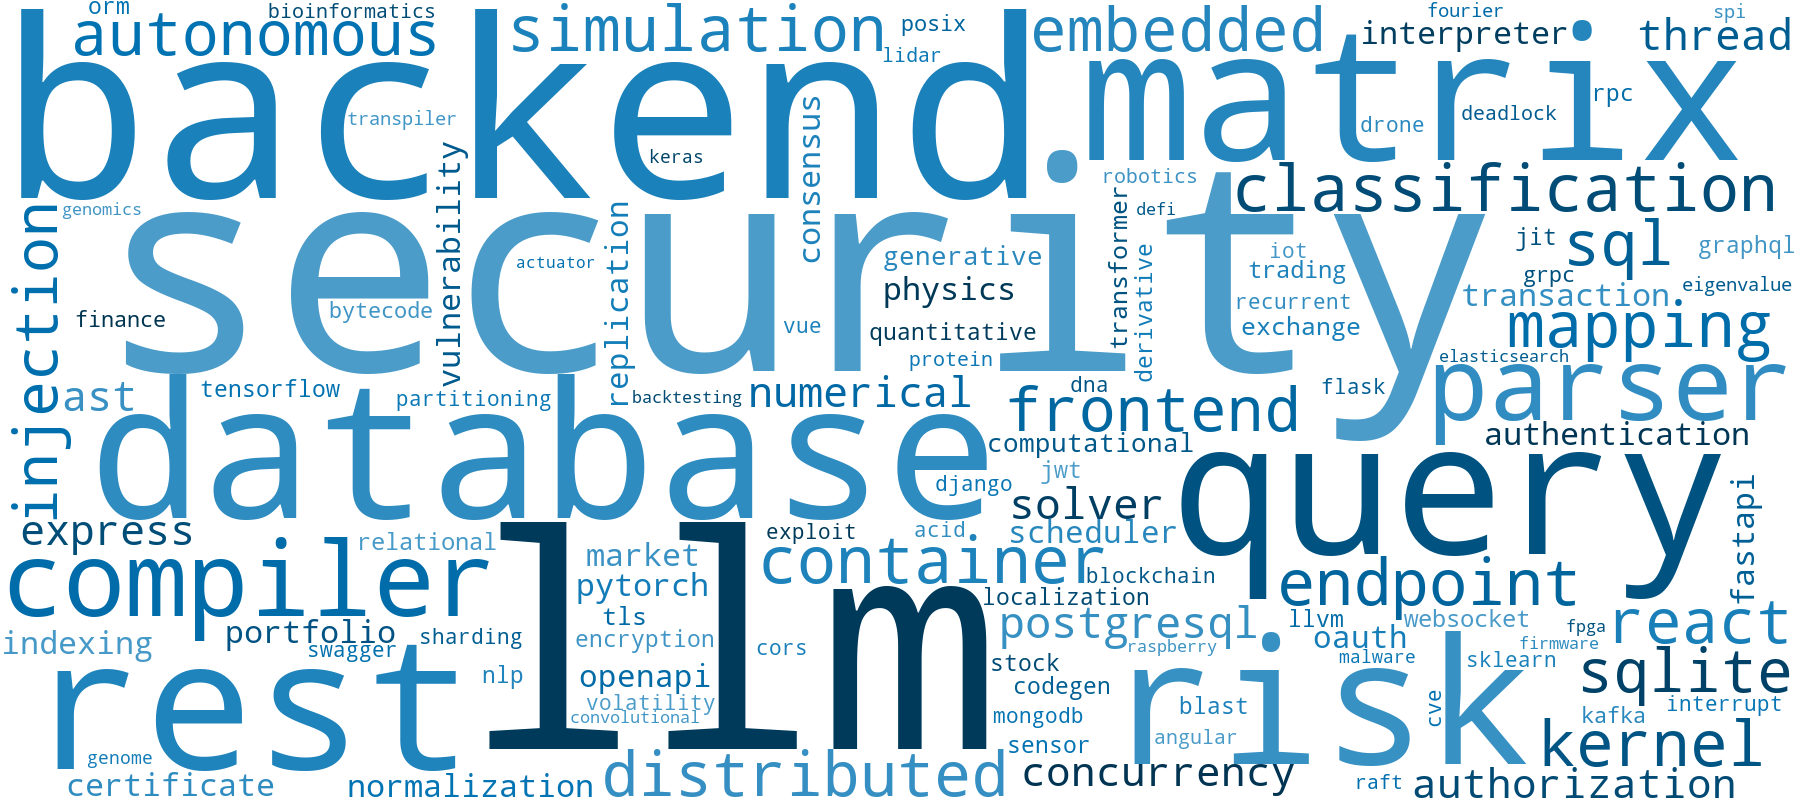
\includegraphics[width=0.92\linewidth]{figures/mt_a7_wordcloud_domain.png}\caption{Domain vocabulary only}\end{subfigure}
\par\medskip
\begin{subfigure}{\linewidth}\centering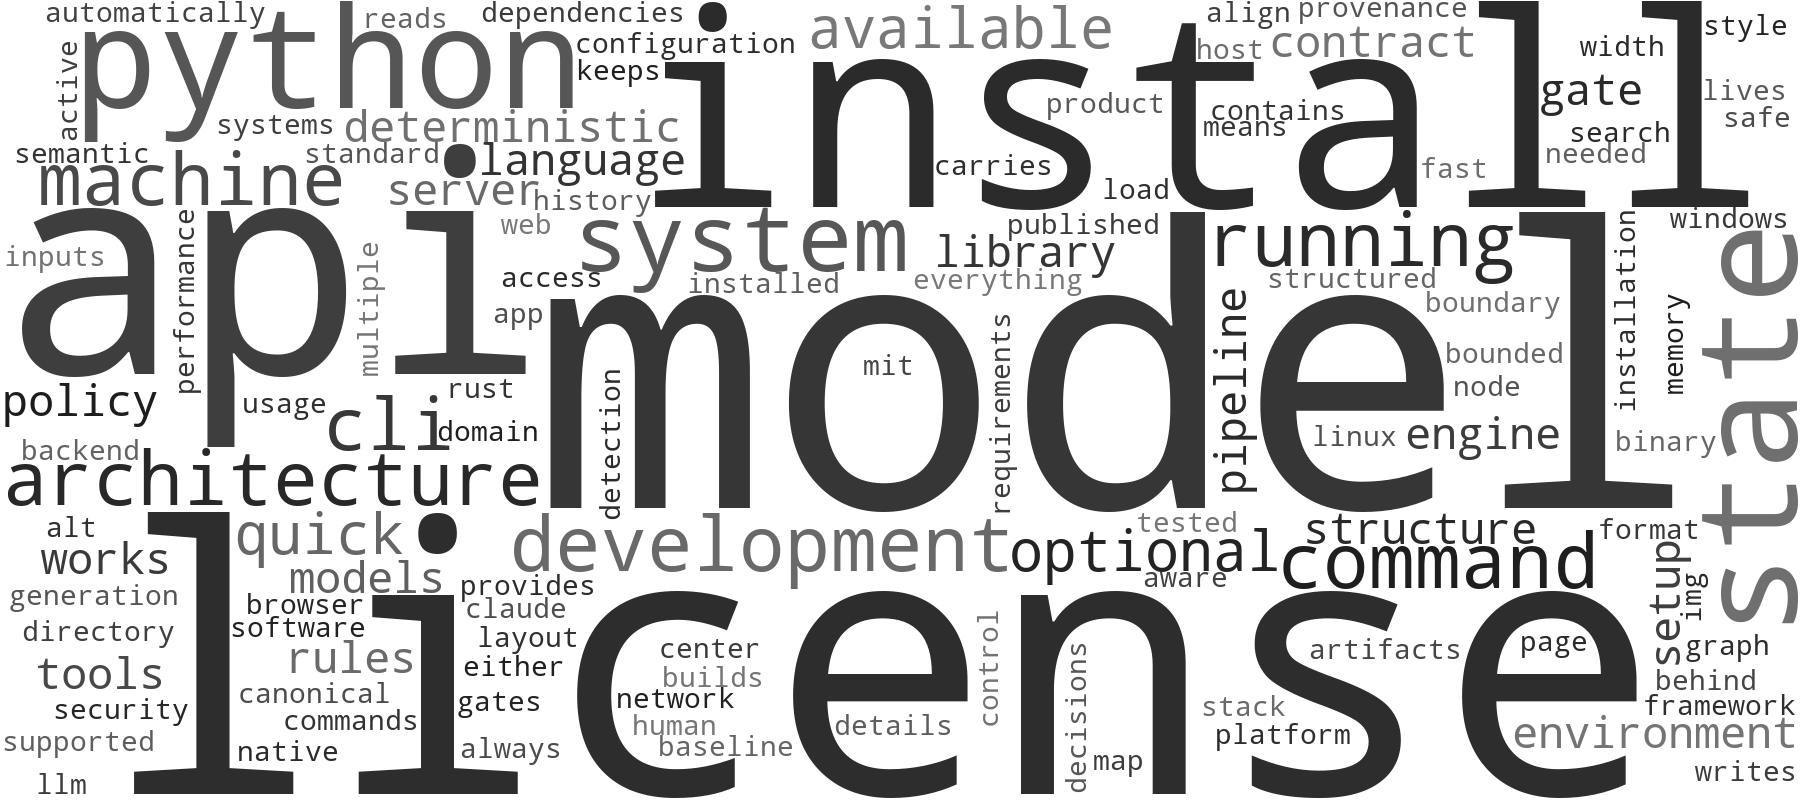
\includegraphics[width=0.92\linewidth]{figures/mt_a7_wordcloud_all.png}\caption{All words (stopwords removed)}\end{subfigure}
\caption{Word clouds of the README and project description of the 1,948 repositories with a verified non-code MT result (A7; 1,809 with a README). Each word counts once per repository; size $\propto \sqrt{\text{repositories}}$.}
\label{fig:mt-a7}
\end{figure}

\paragraph{Repository classification.} \note{Manual classification of the 1,677 usage repositories (actual usage / framework / research artifact / unknown) is in progress (\texttt{usage\_repos\_for\_review.csv}); results to be added.}

\section{RQ3 -- Timeline (commit search)}

Commits are taken from GitHub's commit search (default branches; the whole history is searchable: 64 of 148 sampled repositories had been inactive for over a year). A commit is a \emph{technique commit} if its message contains an MT phrase. Each repository is counted once, in the year of its first technique commit (Figure~\ref{fig:mt-t8}); a commit message mentioning MT does not necessarily mean MT is in the code.

\begin{figure}[htbp]
\centering
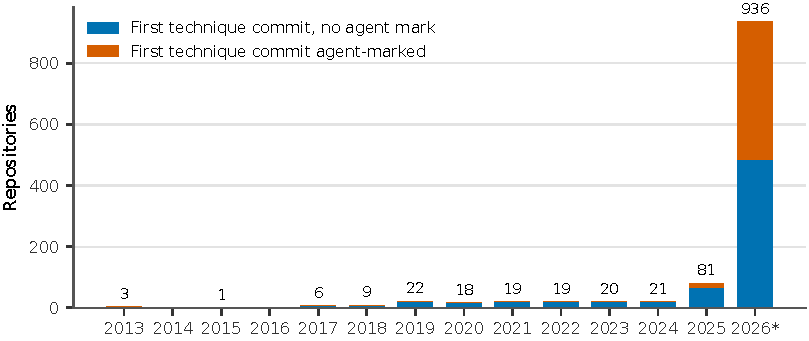
\includegraphics[width=\linewidth]{figures/mt_t8_first_commit.pdf}
\caption{Metamorphic testing: repositories by year of their first commit mentioning the technique (T8), split by whether that commit carries an AI-agent authorship line (e.g.\ \texttt{Co-Authored-By: Claude}; a lower bound). * 2026: January--August.}
\label{fig:mt-t8}
\end{figure}

\paragraph{The 2026 surge.} 937 repositories made their first MT commit in 2026 (to the end of August), against 81 in 2025 and about 20 per year before that. They belong to 849 different owners, 85\% were created in 2026, and 68\% have a single technique commit. 48\% of these first commits, and 59\% of all 3,181 technique commits in 2026, carry an AI-agent authorship line (a lower bound, since several agents leave no trace). The rise is gradual from late 2025 rather than a single burst, and no search artefact explains it (complete search, no concentration in a few accounts, no copied commit messages).

\begin{figure}[htbp]
\centering
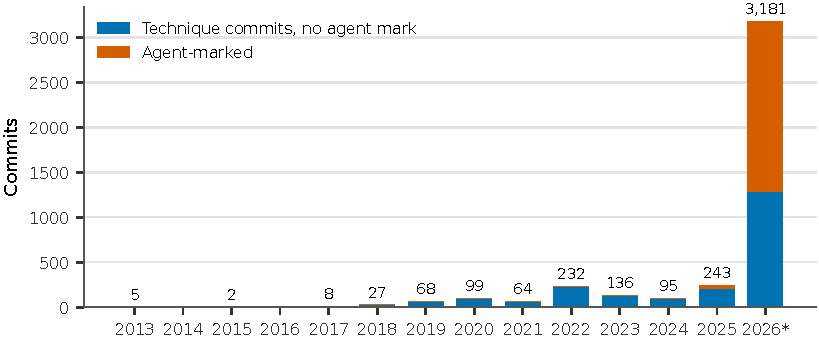
\includegraphics[width=\linewidth]{figures/mt_t9_commits.pdf}
\caption{Metamorphic testing: technique commits per year (T9), with the AI-agent-marked share. * 2026: January--August.}
\label{fig:mt-t9}
\end{figure}

\begin{figure}[htbp]
\centering
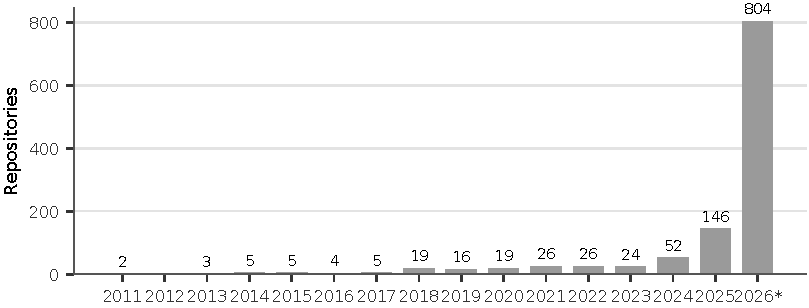
\includegraphics[width=\linewidth]{figures/mt_t8_creation_year.pdf}
\caption{Creation year of the 1,156 repositories with at least one MT commit. * 2026: January--August.}
\label{fig:mt-creation}
\end{figure}

\begin{table}[htbp]
\centering
\small
\caption{Metamorphic testing timeline from the commit search (T8, T9), 2018--2026.}
\label{tab:mt-timeline}
\begin{tabular}{@{}lrrrrrr@{}}
\toprule
Year & \shortstack{First-commit\\repos} & \shortstack{...agent-\\marked} & \shortstack{Technique\\commits} & \shortstack{Agent-\\marked} & Agent \% & \shortstack{Repos with\\commits} \\
\midrule
2018 & 9 & 0 & 27 & 0 & 0\% & 9 \\
2019 & 22 & 0 & 68 & 0 & 0\% & 24 \\
2020 & 18 & 0 & 99 & 0 & 0\% & 26 \\
2021 & 19 & 0 & 64 & 0 & 0\% & 25 \\
2022 & 19 & 0 & 232 & 0 & 0\% & 23 \\
2023 & 20 & 0 & 136 & 0 & 0\% & 30 \\
2024 & 21 & 0 & 95 & 0 & 0\% & 29 \\
2025 & 81 & 14 & 243 & 39 & 16\% & 85 \\
2026 & 937 & 452 & 3,181 & 1,888 & 59\% & 945 \\
\bottomrule
\end{tabular}
\par\smallskip\parbox{0.94\linewidth}{\footnotesize 2026: January--August. Agent-marked: commit message carries an AI-agent authorship line (lower bound).}
\end{table}

\section{Comparison with property-based testing and fuzz testing}

The same pipeline was run for property-based testing (PBT) and fuzz testing, with explicit technique phrases only (no tool or library names). Adoption and timeline are compared below.

\begin{table}[htbp]
\centering
\small
\caption{Adoption: verified repositories per search surface for the three techniques.}
\label{tab:cmp-adoption}
\begin{tabular}{@{}lrrr@{}}
\toprule
Surface & MT & PBT & Fuzz \\
\midrule
Code & 5,879 & $\approx$72,794 $\pm$ 990 & $\approx$233,928 $\pm$ 4,121 \\
Repositories & 230 & 1,205 & 7,050 \\
Commits & 1,156 & 6,710 & 13,355 \\
Pull requests & 507 & 6,555 & 29,251 \\
Issues & 453 & 4,373 & 12,519 \\
Discussions & 8 & 140 & 561 \\
\midrule
Code-surface repositories found by search & 6,117 & 76,846 & 255,740 \\
\bottomrule
\end{tabular}
\par\smallskip\parbox{0.94\linewidth}{\footnotesize MT: every repository verified. PBT, fuzz: code-surface count estimated from the random sample (share of sampled repositories whose current snapshot contains a phrase $\times$ repositories found; $\pm$ 95\% CI). Non-code surfaces of PBT and fuzz are lower bounds: GitHub's 1{,}000-result cap truncated parts of their commit, pull-request and issue searches.}
\end{table}

\begin{figure}[htbp]
\centering
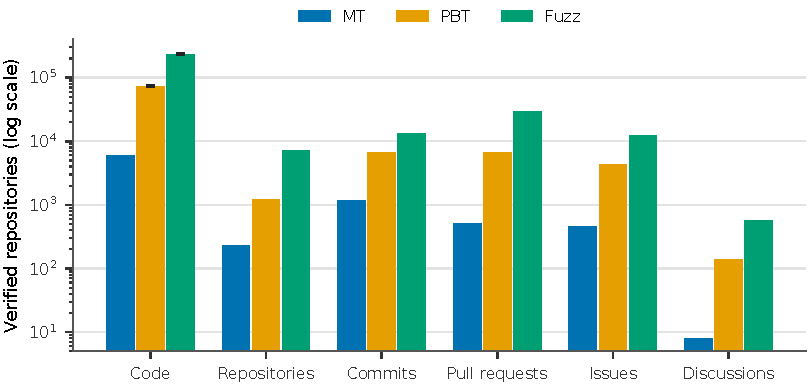
\includegraphics[width=\linewidth]{figures/cmp_repos_per_surface.pdf}
\caption{Verified repositories per search surface (log scale). Code surface of PBT and fuzz: sample estimate with 95\% CI.}
\label{fig:cmp-surfaces}
\end{figure}

\subsection{Project descriptions (A7)}

README and project description of repositories with a verified non-code result: all 1,948 for MT, and the random samples of 1,073 (PBT) and 1,126 (fuzz) repositories. Each word counts once per repository. The domain vocabulary (162 words) is the same for all three techniques, so its word clouds and shares are directly comparable (Table~\ref{tab:cmp-a7}, Figures~\ref{fig:cmp-a7-domain} and~\ref{fig:cmp-a7-all}).

\begin{table}[htbp]
\centering
\small
\caption{Top 15 domain-vocabulary words in the README and description, as a share of repositories (A7).}
\label{tab:cmp-a7}
\begin{tabular}{@{}rlrlrlr@{}}
\toprule
\# & MT & \% & PBT & \% & Fuzz & \% \\
\midrule
1 & llm & 19\% & security & 21\% & security & 22\% \\
2 & security & 17\% & backend & 13\% & database & 10\% \\
3 & backend & 16\% & database & 11\% & container & 10\% \\
4 & database & 14\% & rest & 9\% & backend & 9\% \\
5 & query & 13\% & container & 8\% & compiler & 8\% \\
6 & matrix & 13\% & query & 8\% & distributed & 7\% \\
7 & rest & 12\% & frontend & 8\% & query & 7\% \\
8 & risk & 10\% & distributed & 8\% & authentication & 7\% \\
9 & compiler & 9\% & authentication & 7\% & rest & 6\% \\
10 & parser & 9\% & \textbf{react} & 7\% & \textbf{embedded} & 6\% \\
11 & \textbf{classification} & 9\% & endpoint & 7\% & parser & 5\% \\
12 & container & 9\% & compiler & 6\% & \textbf{kernel} & 5\% \\
13 & endpoint & 8\% & llm & 6\% & risk & 5\% \\
14 & \textbf{mapping} & 8\% & \textbf{postgresql} & 5\% & endpoint & 5\% \\
15 & \textbf{simulation} & 8\% & matrix & 5\% & frontend & 5\% \\
\bottomrule
\end{tabular}
\par\smallskip\parbox{0.94\linewidth}{\footnotesize \% = share of the technique's repositories whose README or description contains the word. \textbf{Bold}: in the top 15 of this technique only. In the top 15 of all three: backend, compiler, container, database, endpoint, query, rest, security.}
\end{table}

\begin{figure}[p]
\centering
\begin{subfigure}{\linewidth}\centering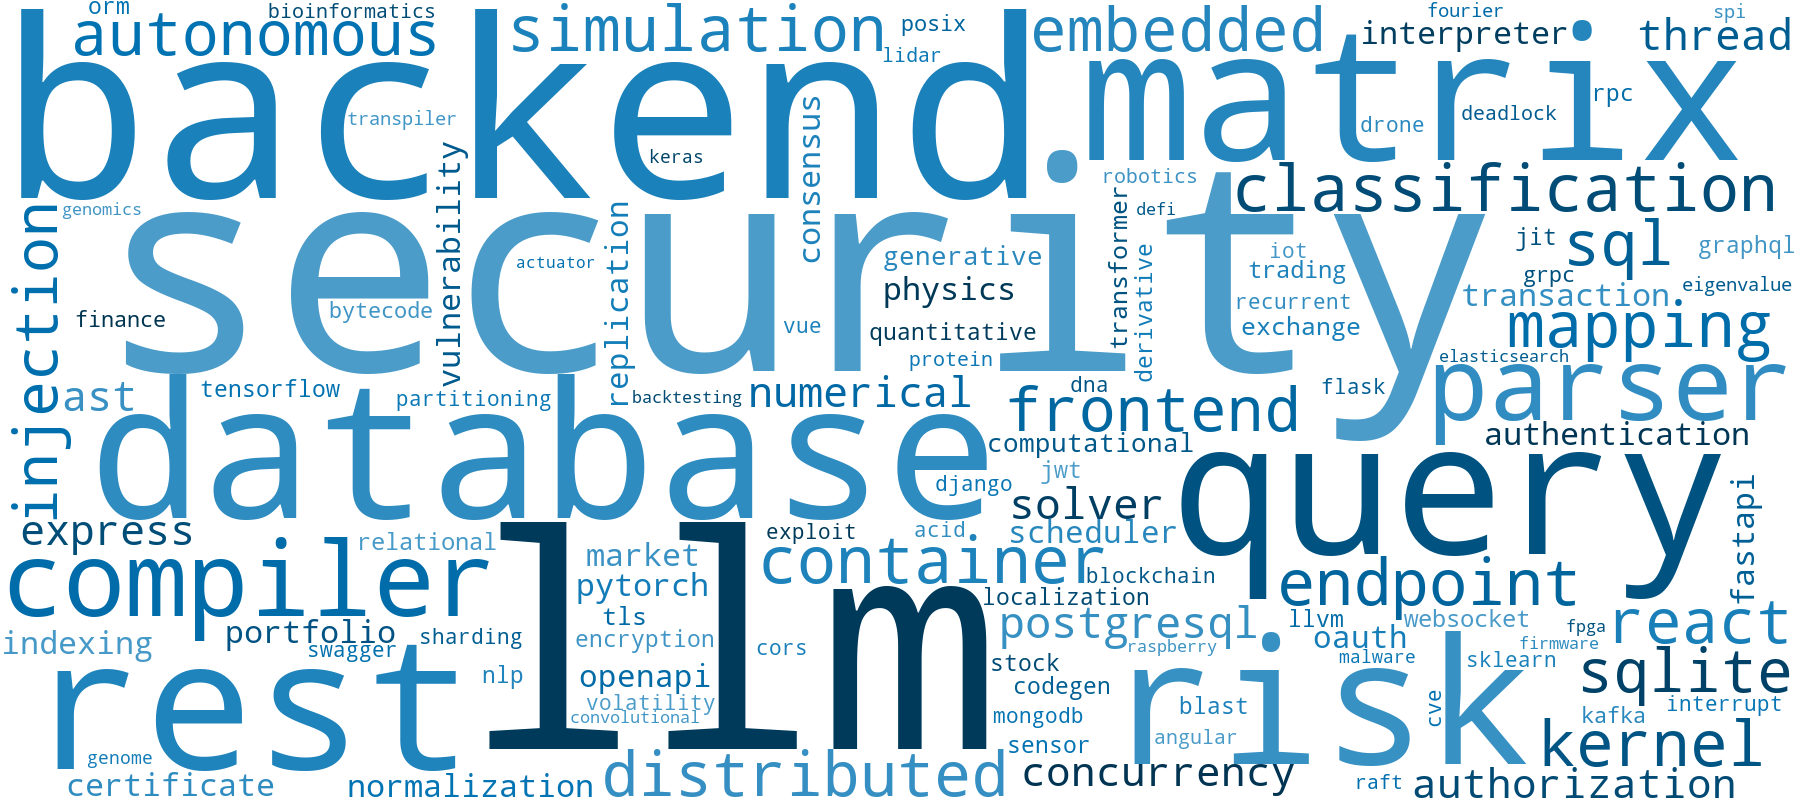
\includegraphics[width=0.86\linewidth]{figures/cmp_a7_whitelist_freq_mt.png}\caption{Metamorphic testing (1,948 repositories)}\end{subfigure}
\par\medskip
\begin{subfigure}{\linewidth}\centering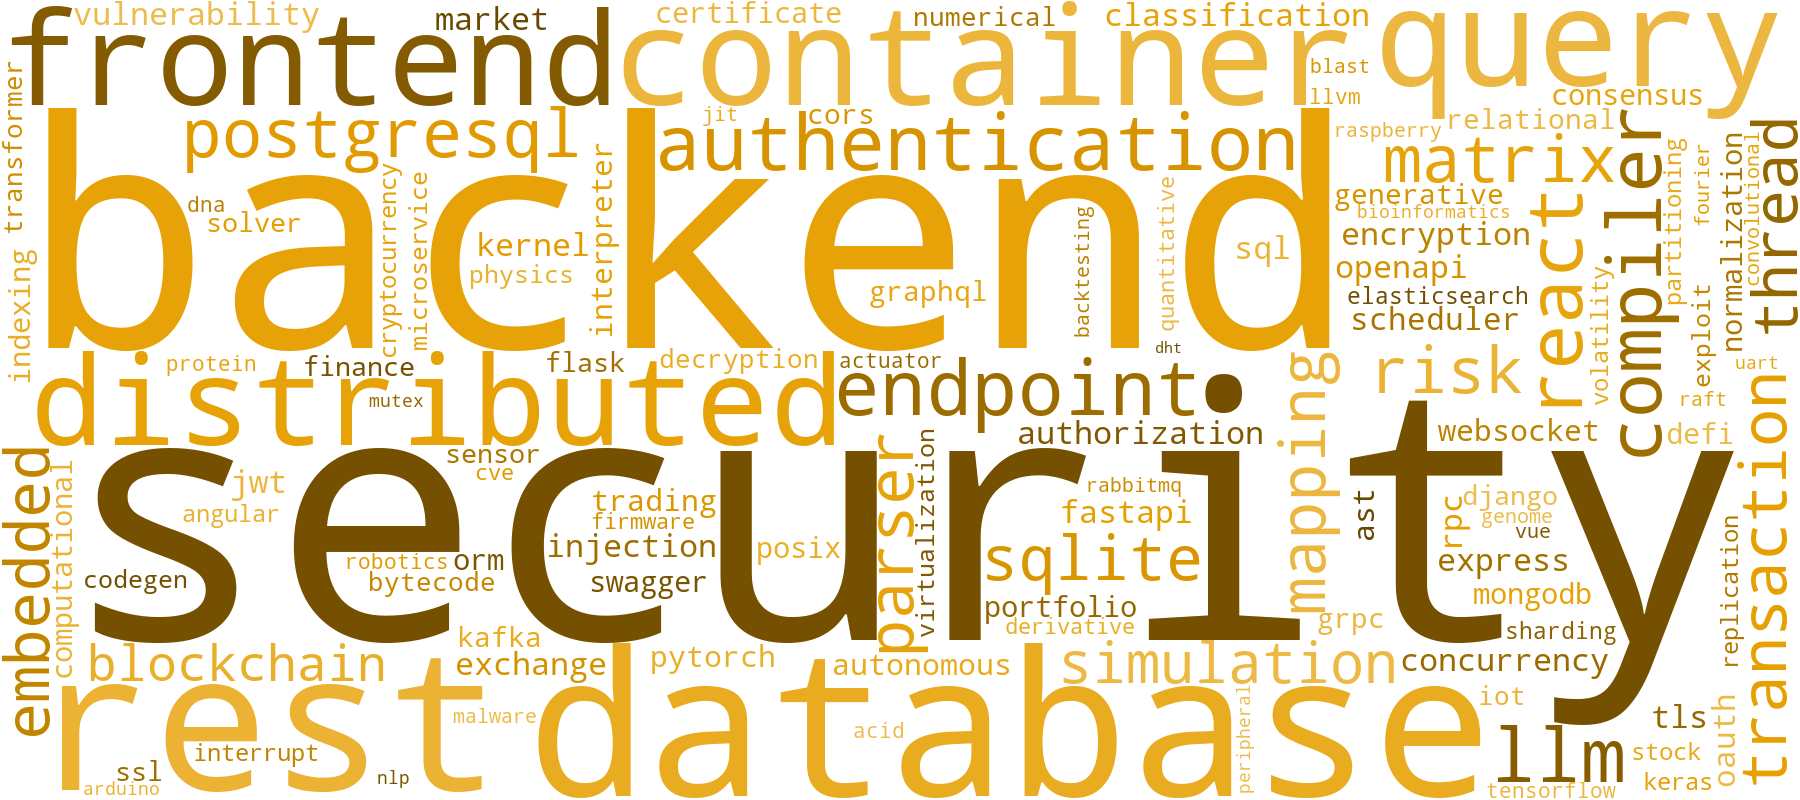
\includegraphics[width=0.86\linewidth]{figures/cmp_a7_whitelist_freq_pbt.png}\caption{Property-based testing (1,073 repositories)}\end{subfigure}
\par\medskip
\begin{subfigure}{\linewidth}\centering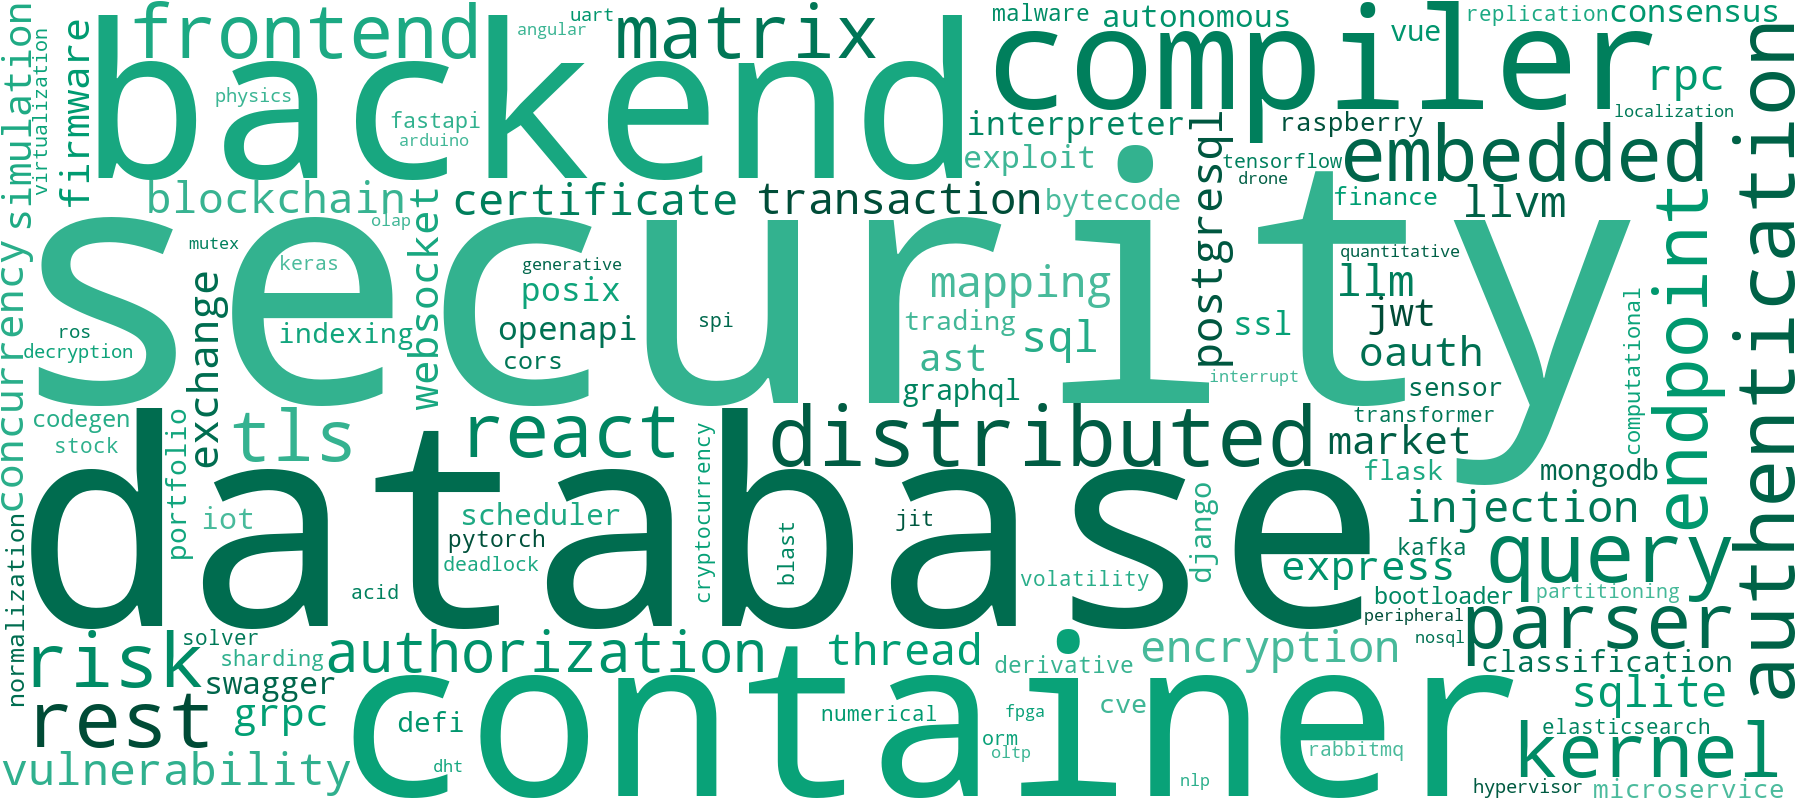
\includegraphics[width=0.86\linewidth]{figures/cmp_a7_whitelist_freq_fuzz.png}\caption{Fuzz testing (1,126 repositories)}\end{subfigure}
\caption{Word clouds of the README and description, domain vocabulary only (A7). Size $\propto \sqrt{\text{repositories}}$.}
\label{fig:cmp-a7-domain}
\end{figure}

\begin{figure}[p]
\centering
\begin{subfigure}{\linewidth}\centering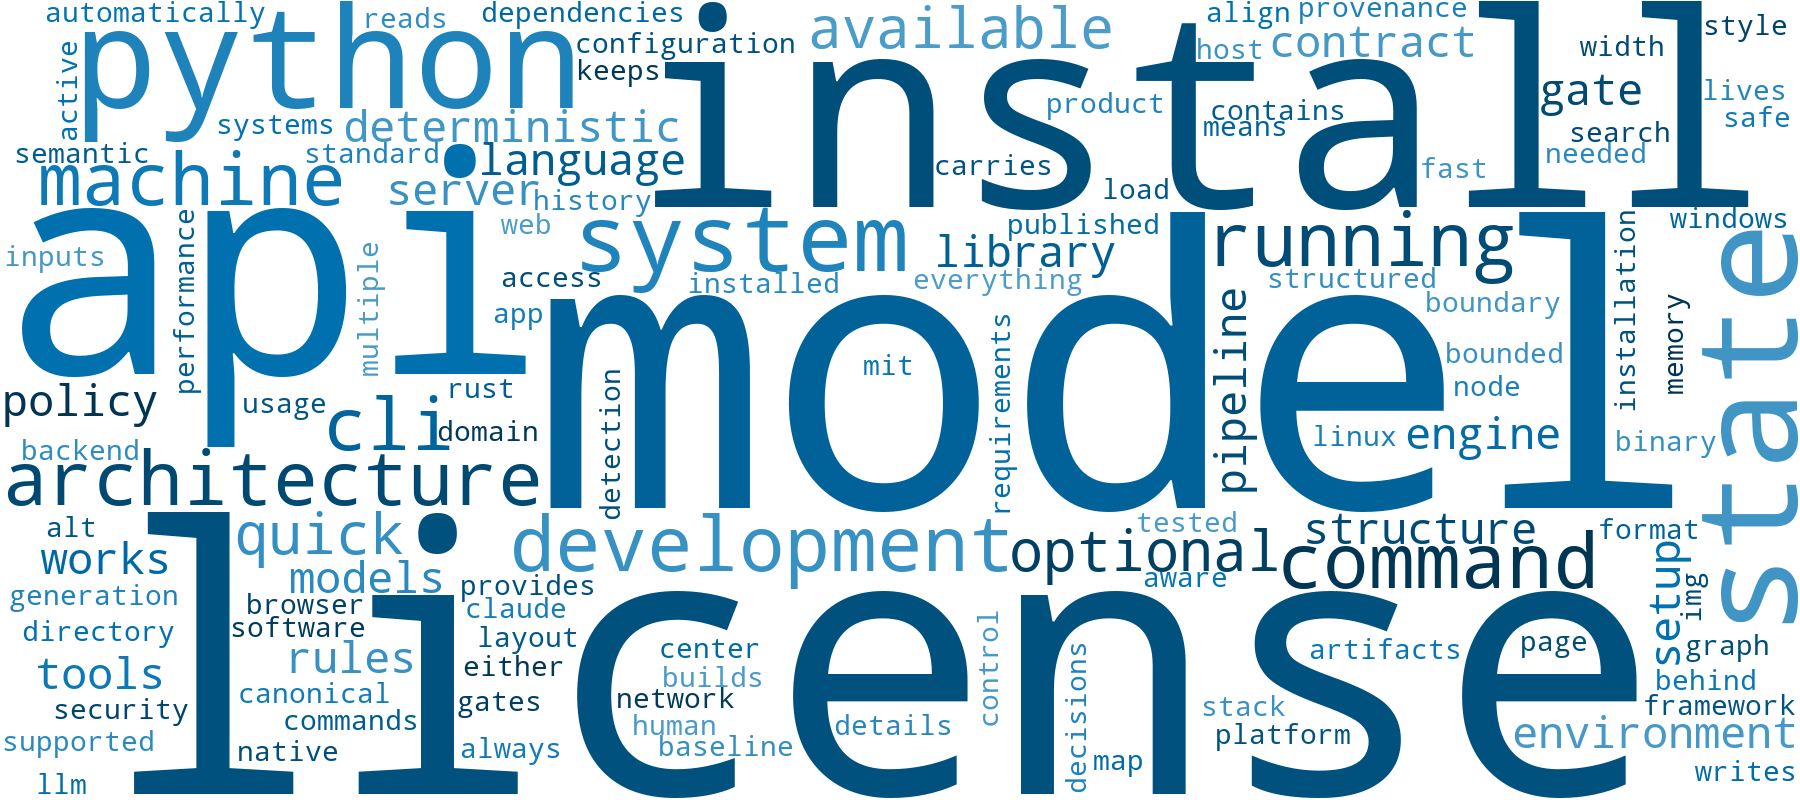
\includegraphics[width=0.86\linewidth]{figures/cmp_a7_freq_mt.png}\caption{Metamorphic testing (1,948 repositories)}\end{subfigure}
\par\medskip
\begin{subfigure}{\linewidth}\centering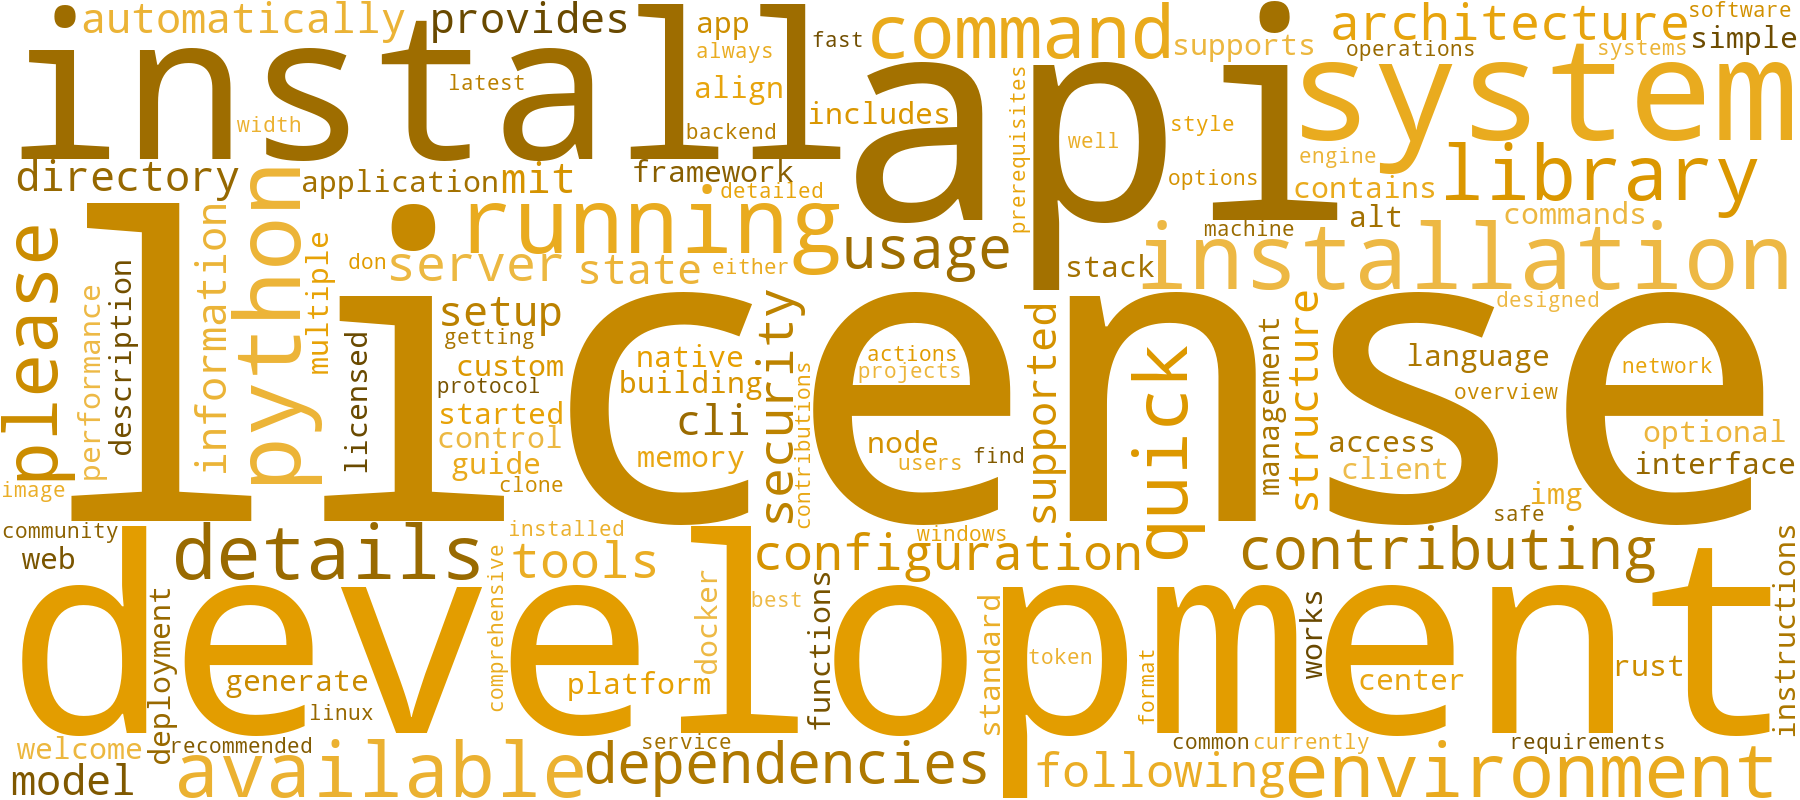
\includegraphics[width=0.86\linewidth]{figures/cmp_a7_freq_pbt.png}\caption{Property-based testing (1,073 repositories)}\end{subfigure}
\par\medskip
\begin{subfigure}{\linewidth}\centering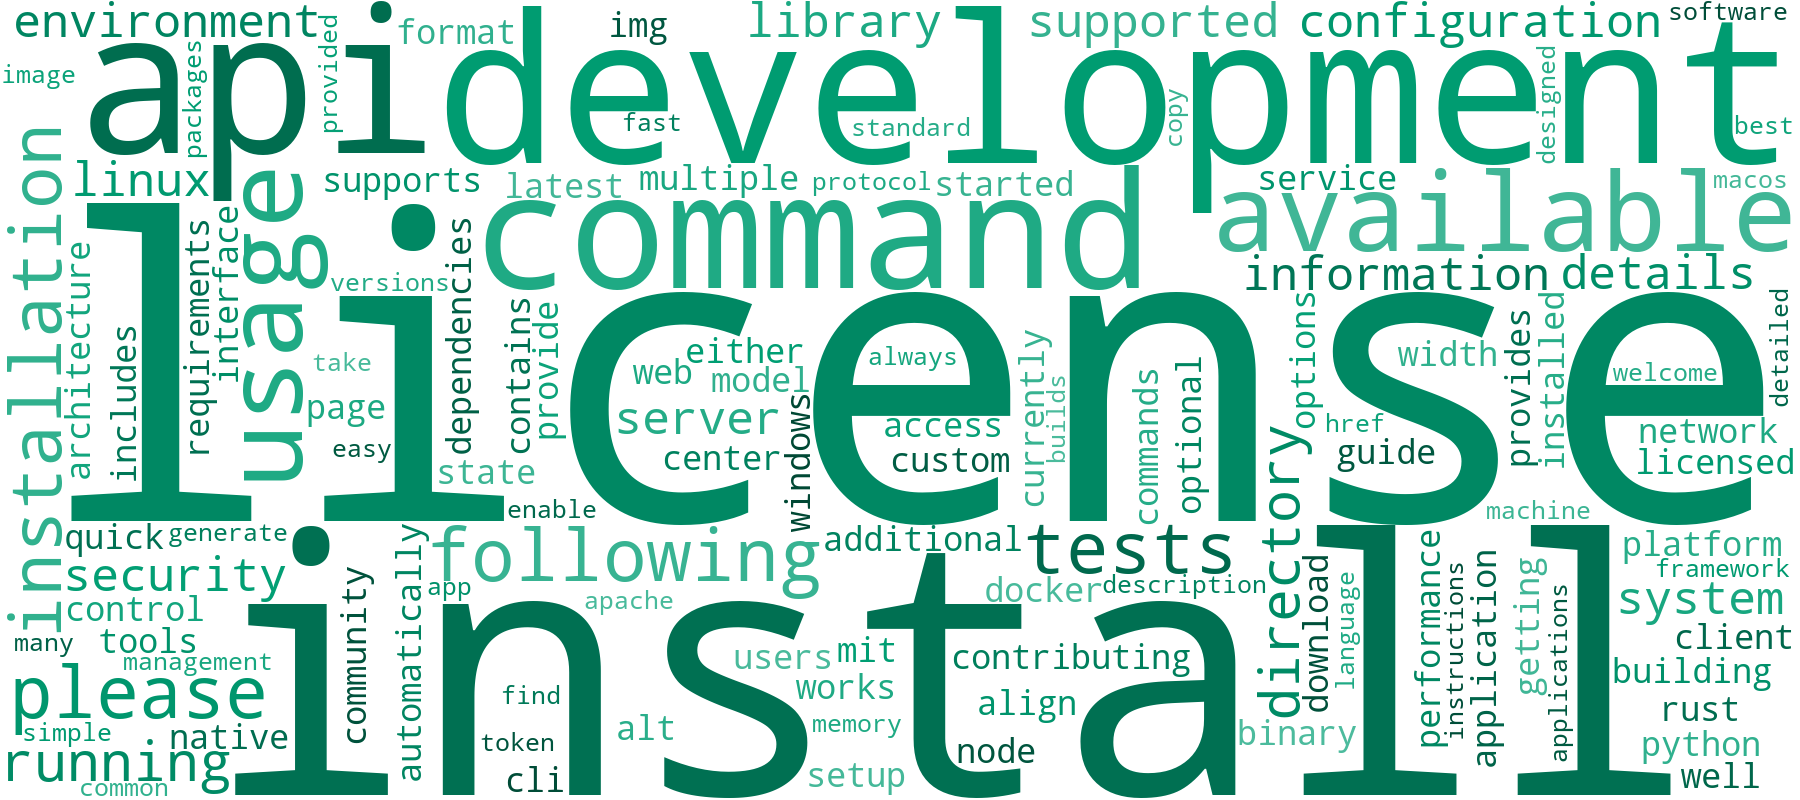
\includegraphics[width=0.86\linewidth]{figures/cmp_a7_freq_fuzz.png}\caption{Fuzz testing (1,126 repositories)}\end{subfigure}
\caption{Word clouds of the README and description, all words (stopwords removed; A7). Size $\propto \sqrt{\text{repositories}}$.}
\label{fig:cmp-a7-all}
\end{figure}

\begin{figure}[htbp]
\centering
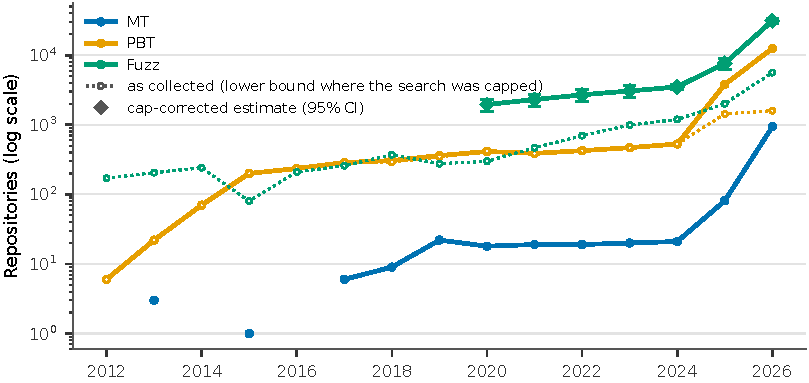
\includegraphics[width=\linewidth]{figures/cmp_first_commit_per_year.pdf}
\caption{Repositories by year of their first commit mentioning the technique (log scale). Solid: counts corrected for GitHub's 1{,}000-result cap (PBT: exact recount; fuzz: random-window estimate with 95\% CI where available); dotted: as collected. 2026: January--August.}
\label{fig:cmp-first-commit}
\end{figure}

\begin{table}[htbp]
\centering
\small
\caption{Timeline comparison: repositories by year of first technique commit, and AI-agent-marked share of technique commits.}
\label{tab:cmp-timeline}
\begin{tabular}{@{}lrrrrrr@{}}
\toprule
 & \multicolumn{3}{c}{First-commit repositories} & \multicolumn{3}{c}{Agent-marked share} \\ \cmidrule(lr){2-4}\cmidrule(lr){5-7}
Year & MT & PBT & Fuzz & MT & PBT & Fuzz \\
\midrule
2020 & 18 & 413 & 1,955 $\pm$ 382 & 0\% & 0\% & 0\% $\pm$ 0 \\
2021 & 19 & 388 & 2,304 $\pm$ 445 & 0\% & 0\% & 0\% $\pm$ 0 \\
2022 & 19 & 425 & 2,695 $\pm$ 528 & 0\% & 0\% & 0\% $\pm$ 1 \\
2023 & 20 & 469 & 3,062 $\pm$ 565 & 0\% & 0\% & 0\% $\pm$ 0 \\
2024 & 21 & 529 & 3,500 $\pm$ 286 & 0\% & 0\% & 0\% $\pm$ 0 \\
2025 & 81 & 3,796 & 7,642 $\pm$ 1,323 & 16\% & 23\% & 5\% $\pm$ 1 \\
2026 & 937 & 12,479 & 31,180 $\pm$ 2,471 & 59\% & 31\% & 27\% $\pm$ 2 \\
\bottomrule
\end{tabular}
\par\smallskip\parbox{0.94\linewidth}{\footnotesize 2026: January--August. PBT: exact recount of the capped commit-search ranges. Fuzz: $\pm$ = 95\% CI of the random-window estimate; $^{\dagger}$ as collected, a lower bound for fuzz (its commit search was capped in every year).}
\end{table}

\begin{figure}[htbp]
\centering
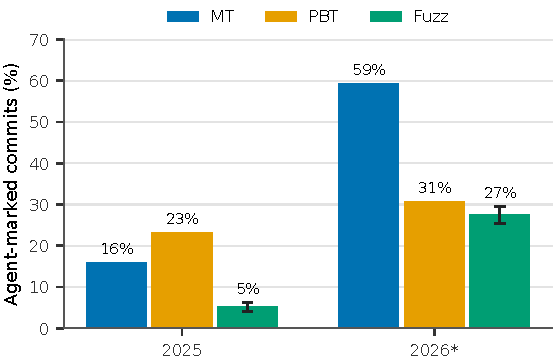
\includegraphics[width=0.68\linewidth]{figures/cmp_agent_share.pdf}
\caption{Share of technique commits with an AI-agent authorship line (lower bound), 2025 and 2026 (January--August). Fuzz: estimate with 95\% CI.}
\label{fig:cmp-agent}
\end{figure}

\end{document}
